\documentclass[man,natbib,floatsintext]{apa6} %apa 6th edition format

% watermark for first page
% \usepackage[firstpage]{draftwatermark}
% \SetWatermarkText{In Prep}
% \SetWatermarkScale{.75}
% \SetWatermarkColor[gray]{0.88}

\usepackage{amstext,amssymb,graphicx,bm,soul,color,url,lscape,rotating,setspace,csquotes,pdflscape,rotating}
% \DeclareDelayedFloatFlavor{sidewaystable}{table}
% \DeclareDelayedFloatFlavor{sidewaysfigure}{figure}


\usepackage[space]{grffile}

% as setup by apacite, natbib puts extra spaces between the commas and semicolons in the cites. This fixes it:
\setcitestyle{citesep={;},aysep={,}}
 
% Run texcount on tex-file and write results to a file
\newcommand\wordcount{\input{wordcount.sum}}

% environment to display a page in landscape in the final pdf
\newenvironment{rotatepage}%
    {\pagebreak[4]\global\pdfpageattr\expandafter{\the\pdfpageattr/Rotate 180}}%
    {\pagebreak[4]\global\pdfpageattr\expandafter{\the\pdfpageattr/Rotate 0}}%

% commands for inserting values determined by analyses scripts.
\newcommand\shoeExplicit{290}
\newcommand\shoeIncidental{386}
\newcommand\doorExplicit{137}
\newcommand\doorIncidental{255}
\newcommand\Movie{384}
\newcommand\Relational{409}
\newcommand\Scenario{331}
\newcommand\Animacy{325}
\newcommand\Weight{322}
\newcommand\shoeExplicitAware{--}
\newcommand\shoeIncidentalAware{47}
\newcommand\doorExplicitAware{--}
\newcommand\doorIncidentalAware{43}
\newcommand\MovieAware{55}
\newcommand\RelationalAware{98}
\newcommand\ScenarioAware{32}
\newcommand\AnimacyAware{31}
\newcommand\WeightAware{31}
\newcommand\shoeExplicitIncluded{290}
\newcommand\shoeIncidentalIncluded{339}
\newcommand\doorExplicitIncluded{137}
\newcommand\doorIncidentalIncluded{212}
\newcommand\MovieIncluded{329}
\newcommand\RelationalIncluded{311}
\newcommand\ScenarioIncluded{299}
\newcommand\AnimacyIncluded{294}
\newcommand\WeightIncluded{291}
\newcommand\shoeExplicitPrec{0.46 (0.16)}
\newcommand\shoeIncidentalPrec{0.40 (0.16)}
\newcommand\doorExplicitPrec{0.47 (0.17)}
\newcommand\doorIncidentalPrec{0.47 (0.14)}
\newcommand\MoviePrec{0.38 (0.15)}
\newcommand\RelationalPrec{0.44 (0.18)}
\newcommand\ScenarioPrec{0.38 (0.14)}
\newcommand\AnimacyPrec{0.37 (0.14)}
\newcommand\WeightPrec{0.42 (0.15)}


% counter for panels of crp matrix figure
\newcounter{crppanel}

% commands for making margin notes marked with authors initials
\setlength{\marginparwidth}{30pt}
\newcommand{\mkh}[1]{\marginpar{\scriptsize \textcolor{red}{MKH: #1}}}

\title{Supplemental Methods for: Temporal Contiguity in Incidentally Encoded Memories} 

\author{M.\ Karl Healey}

\affiliation{Michigan State University}

\shorttitle{Supplemental Methods: Contiguity with Incidental Encoding}

\keywords{episodic memory; free recall; temporal contiguity}

\begin{document}
\maketitle


% setup some commands to make changing text from study to study easy
\newcommand\listlength{16} % words per list 
\newcommand\presrate{4 seconds} % time per word
\newcommand\isi{1 second} %
\newcommand\DFRDelay{16 seconds} % length of distractor at end of study
\newcommand\recalltime{75 seconds} % time to recall
\newcommand\totalss{XX}
\newcommand\totalexcluded{XX}

\section{Encoding Instructions Manipulation} In Experiments 1 and 2, subjects were randomly assigned to either the Incidental condition or the Explicit condition. Prior to seeing the first list, subjects in both conditions were told that they would see a series of words and would make a simple judgment about each one. The exact instructions depended on the condition. In the Explicit condition, subjects were given standard free recall instructions that described the judgment task but emphasized memory. Because the wording of the instructions are integral to the intent manipulation, they are quoted directly here:
\textbf{Explicit Instructions:}

\begin{displayquote}
        Thank you for participating in this study. 

        We are interested in how people make simple judgments about common words and
        how they subsequently remember the words. Please position this window in the center
        of your screen so you can comfortably view the words.

        You will see a list of words appear one at a time and make a judgment about each one
        (more details on the next page). After the list of words, you will do a few math problems.
        After the math problems, you will be prompted to type in any words that you can remember
        from the list.

        When prompted, type any words that you can remember from the list you just saw,
        \emph{in any order} (type one word in each of the provided text boxes).

    [\textit{a screen showing task instructions, which did not mention memory and was identical for both conditions}]

        Your main task is to remember as many of the words as possible; at the end of the list you will be prompted to
    type as many words as you can remember from the list you just saw, \emph{in any order}.
\end{displayquote}


\textbf{Incidental Instructions:}

\begin{displayquote}
        Thank you for participating in this study.

        We are interested in how people make simple judgments about common words.
        Please position this window in the center of your screen so you can comfortably view the words.

        You will see a list of words appear one at a time and make a judgment about each one
        (more details on the next page). After the list of words, you will do a few math problems.
        
        [\textit{a screen showing task instructions, which did not mention memory and was identical for both conditions}]

        Your main task is to make as accurate a judgment as possible about each word.
\end{displayquote}

\section{Judgment Tasks} 
In all conditions across all three Experiments, subjects were asked to make a judgment about each word while it was present on the screen. Because subjects completed the task online and could not ask an experimenter for clarification, several measures were taken to ensure that subjects understood how to make a response and could be confident that their responses were being registered: During presentation of the lists, a task prompt was displayed above each word (e.g., ``Is it easy to judge if it would it fit in a shoebox?''). An instruction about how to make a response was displayed below each word (i.e., ``press ``Y'' for yes, ``N'' for no''). The task prompt and response instructions were in lighter gray font than the black font used for words. The prompts disappeared once the subject made a valid response, but if the subject made an invalid response (e.g., pressing ``B'' instead of ``Y'' or ``N'') the response instructions were replaced with an error message in red font until a valid response was made. The word remained on screen for the full presentation period regardless of the subject's response.

The exact instructions for each judgment tasks were:

\subsection{Shoebox Task}
\begin{displayquote}
We are trying to find a set of words that are neither too easy nor too hard for people to process. We want to use these words in an upcoming study of brain activity during word processing. Your responses today will help us select appropriate words.

You will be asked to make a judgment about each word in the list. Specifically, you will decide whether or not the word refers to an object that could fit into a regular shoebox.

You will see each word for only a few seconds. Therefore, for some words, you will find it easy to decide if it fits in a shoebox. For other words, you will find it difficult. For each word, you will try to decide if it fits in a shoebox and indicate whether it was easy or difficult.

There are two possible choices for each word: "Yes" and "No". You will respond by pressing the "y" key for "Yes" or the "n" key for "No".

For example, if we asked you to judge the word "owner", you would press "y" if you can easily decide if it fits in a shoebox, and "n" if you find it difficult.

The task will automatically advance to the next word after a fixed amount of time. There will be a brief screen showing a cross, "+", between each word presentation.
To ensure participants are thinking carefully about each word, we will randomly pause the task and ask you to type a description of how you made your judgment.
\end{displayquote}



\subsection{Front Door Task}
\begin{displayquote}
We are trying to find a set of words that are neither too easy nor too hard for people to process. We want to use these words in an upcoming study of brain activity during word processing. Your responses today will help us select appropriate words.

You will be asked to make a judgment about each word in the list. Specifically, for each word, you will think of the object it refers to and try to imagining yourself moving that object through the front door of your home. Ask yourself if the object would successfully fit through your front door.

You will see each word for only a few seconds. Therefore, for some words, you will find it easy to decide if it would fit through your front door. For other words, you will find it difficult. For each word, you will try to decide if it would fit through your front door and indicate whether it was easy or difficult.

There are two possible choices for each word: "Yes" and "No". You will respond by pressing the "y" key for "Yes" or the "n" key for "No".

For example, if we asked you to judge the word "owner", you would press "y" if you can easily decide if would fit through your front door, and "n" if you find it difficult.

The task will automatically advance to the next word after a fixed amount of time. There will be a brief screen showing a cross, "+", between each word presentation.
To ensure participants are thinking carefully about each word, we will randomly pause the task and ask you to type a description of how you made your judgment.
\end{displayquote}

\subsection{Weight Task}
\begin{displayquote}
We are trying to find a set of words that are neither too easy nor too hard for people to process. We want to use these words in an upcoming study of brain activity during word processing. Your responses today will help us select appropriate words.

You will be asked to make a judgment about each word in the list. Specifically, you will decide whether or not the word refers to an object that is heavier than a standard bottle of water you'd purchase from a vending machine.

You will see each word for only a few seconds. Therefore, for some words, you will find it easy to decide if it is heavier than a bottle of water. For other words, you will find it difficult. For each word, you will think about its weight and try to decide if it is heavier than a bottle of water and indicate whether it was easy or difficult.

There are two possible choices for each word: "Yes" and "No". You will respond by pressing the "y" key for "Yes" or the "n" key for "No".

For example, if we asked you to judge the word "owner", you would press "y" if you can easily decide if it is heavier than a bottle of water, and "n" if you find it difficult.

The task will automatically advance to the next word after a fixed amount of time. There will be a brief screen showing a cross, "+", between each word presentation.
To ensure participants are thinking carefully about each word, we will randomly pause the task and ask you to type a description of how you made your judgment.
\end{displayquote}

\subsection{Animacy Task}
\begin{displayquote}
We are trying to find a set of words that are neither too easy nor too hard for people to process. We want to use these words in an upcoming study of brain activity during word processing. Your responses today will help us select appropriate words.

You will be asked to make a judgment about each word in the list. Specifically, you will decide whether or not the word refers to something that is alive.

You will see each word for only a few seconds. Therefore, for some words, you will find it easy to decide if it is something that is alive. For other words, you will find it difficult. For each word, you will try to decide if it is something that is alive and indicate whether it was easy or difficult.

There are two possible choices for each word: "Yes" and "No". You will respond by pressing the "y" key for "Yes" or the "n" key for "No".

For example, if we asked you to judge the word "owner", you would press "y" if you can easily decide if it is alive, and "n" if you find it difficult.

The task will automatically advance to the next word after a fixed amount of time. There will be a brief screen showing a cross, "+", between each word presentation.
To ensure participants are thinking carefully about each word, we will randomly pause the task and ask you to type a description of how you made your judgment.
\end{displayquote}

\subsection{Survival Scenario Task}
\begin{displayquote}
We are trying to find a set of words that are neither too easy nor too hard for people to process. We want to use these words in an upcoming study of brain activity during word processing. Your responses today will help us select appropriate words.

You will be asked to make a judgment about each word in the list. Specifically, you will decide how relevant each word is to an imaginary scenario.

We would like you to imagine that you are planning to move to a new home in a foreign land. Over the next few months, you'll need to purchase a new house and find help transporting your belongings.

For each word you see, think of how relevant the word would be for you in this moving situation. Some of the words may be relevant and others may not it's up to you to decide.

You will see each word for only a few seconds. Therefore, for some words, you will find it easy to judge its relevance. For other words, you will find it difficult. For each word, you will try to judge its relevance and decide if it is easy or difficult.

There are two possible choices for each word: "Yes" and "No". You will respond by pressing the "y" key for "Yes" or the "n" key for "No".

For example, if we asked you to judge the word "owner", you would press "y" if you can easily judge its relevance, and "n" if you find it difficult.

The task will automatically advance to the next word after a fixed amount of time. There will be a brief screen showing a cross, "+", between each word presentation.

To ensure participants are thinking carefully about each word, we will randomly pause the task and ask you to type a description of how you made your judgment.
\end{displayquote}

\subsection{Movie Task}
\begin{displayquote}
We are trying to find a set of words that are neither too easy nor too hard for people to process. We want to use these words in an upcoming study of brain activity during word processing. Your responses today will help us select appropriate words.

You will be asked to make a judgment about each word in the list. Specifically, you will decide whether or not you can easily generate a ``mental movie'' related to that word.

When you read a word, it can trigger many different thoughts. For example, if you see the word ``BASEBALL'' you might have a mental image of a baseball, you might hear the crack of a bat hitting a ball, you might think of related concepts like ballpark, players, and fans. You might have a mental image of a baseball game that includes the sounds, sights, and smells of a baseball stadium. You might think back to personal experiences related to baseball such as the last time you watched a game, or learning to play baseball as a child. All of these thoughts may be associated with positive or negative emotions.

For each word you see, allow it to activate as many different thoughts as possible. Then use these thoughts to generate a mental movie (like a detailed image of spending an afternoon at a baseball game or what it is like to be a player on a baseball field).

You will see each word for only a few seconds. Therefore, for some words, you will find it easy to generate a mental movie. For other words, you will find it difficult. For each word, you will try to form a mental movie and decide if it is easy or difficult.

There are two possible choices for each word: "Yes" and "No". You will respond by pressing the "y" key for "Yes" or the "n" key for "No".

For example, if we asked you to judge the word "owner", you would press "y" if you can easily generate a scene, and "n" if you find it difficult.

The task will automatically advance to the next word after a fixed amount of time. There will be a brief screen showing a cross, "+", between each word presentation.

To ensure participants are thinking carefully about each word, we will randomly pause the task and ask you to type a description of your mental movie.
\end{displayquote}

\subsection{Relational Movie Task}
\begin{displayquote}
We are trying to find a set of words that are neither too easy nor too hard for people to process. We want to use these words in an upcoming study of brain activity during word processing. Your responses today will help us select appropriate words.

You will be asked to make a judgment about each word in the list. Specifically, you will decide whether or not you can easily incorporate each word into an ongoing ``mental movie''.

When you read a word, it can trigger many different thoughts. For example, if you see the word ``BASEBALL'' you might have a mental image of a baseball, you might hear the crack of a bat hitting a ball, you might think of related concepts like ballpark, players, and fans. You might have a mental image of a baseball game that includes the sounds, sights, and smells of a baseball stadium. You might think back to personal experiences related to baseball such as the last time you watched a game, or learning to play baseball as a child. All of these thoughts may be associated with positive or negative emotions.

For each word you see, allow it to activate as many different thoughts as possible. Then use these thoughts to generate a mental movie (like a detailed image of spending an afternoon at a baseball game or what it is like to be a player on a baseball field).

Critically, try to incorporate each new word into your existing mental movie. For example, if the next word was "owner", you should allow it to activate many associated thoughts and then incorporate it into your existing ``ballpark'' movie. You might think of, for example, the owner of a ballpark, of the owners box in the stadium, of a person in a business suit, of a person negotiating a deal to buy a baseball team.

You will see each word for only a few seconds. Therefore, for some words, you will find it easy to incorporate it into your mental movie. For other words, you will find it difficult. For each word, you will try to incorporate it into your mental movie and decide if it is easy or difficult.

There are two possible choices for each word: "Yes" and "No". You will respond by pressing the "y" key for "Yes" or the "n" key for "No".

For example, if we asked you to judge the word "owner", you would press "y" if you can easily incorporate it into your movie, and "n" if you find it difficult.

The task will automatically advance to the next word after a fixed amount of time. There will be a brief screen showing a cross, "+", between each word presentation.

To ensure participants are thinking carefully about each word, we will randomly pause the task and ask you to type a description of your mental movie.
\end{displayquote}



\subsection{Constant Size Task}
\begin{displayquote}
We are trying to find a set of words that are neither too easy nor too hard for people to process. We want to use these words in an upcoming study of brain activity during word processing. Your responses today will help us select appropriate words.

     You will be asked to make a judgment about each word in the list.
       Specifically, you will decide whether or not the word refers to an object that is larger than a regular shoebox.

       You will see each word for only a few seconds. Therefore, for some words, you will find it easy to
           decide if it is larger than a shoebox. For other words, you will find it difficult.
           For each word, you will try to decide if it is larger than a shoebox and indicate whether it was easy or difficult.

      There are two possible choices for each word: "Yes" and "No". You will respond by pressing
      the "y" key for "Yes" or the "n" key for "No".

      For example, if we asked you to judge the word "owner", you would press "y" if you can easily decide
          if is larger than a shoebox, and "n" if you find it difficult.

      The task will automatically advance to the next word after a fixed amount of time.
      There will be a brief screen showing a cross, "+", between each word presentation.

      To ensure participants are thinking carefully about each word, we will
          randomly pause the task and ask you to type a description of how you made your judgment.
\end{displayquote}


\subsection{Varying Size Task}
\begin{displayquote}
We are trying to find a set of words that are neither too easy nor too hard for people to process. We want to use these words in an upcoming study of brain activity during word processing. Your responses today will help us select appropriate words.

       You will be asked to make a judgment about each word in the list.
       Specifically, you will decide whether or not the word refers to an object that is larger than a some other reference object.
           The specific reference object you are comparing the word to will be shown on the screen and will vary from word to word.

       You will see each word for only a few seconds. Therefore, for some words, you will find it easy to
           decide if it is larger than the reference object. For other words, you will find it difficult.
           For each word, you will try to decide if it is larger than the reference object and indicate whether it was easy or difficult.

      There are two possible choices for each word: "Yes" and "No". You will respond by pressing
      the "y" key for "Yes" or the "n" key for "No".

      For example, if we asked you to judge the word "owner" aginst the reference object "shoebox", you would press "y" if you can easily decide
          if is larger than a shoebox, and "n" if you find it difficult.

      The task will automatically advance to the next word after a fixed amount of time.
      There will be a brief screen showing a cross, "+", between each word presentation.

      To ensure participants are thinking carefully about each word, we will
          randomly pause the task and ask you to type a description of how you made your judgment.
\end{displayquote}
The size refereents were randomly choosen from the following (none of which were in the pool of words used to create the item lists):
tennis ball; bowling ball; postage stamp; key; penny; dollar bill; credit card; 2-liter bottle; gallon of milk; lightbulb; cell phone; coffee mug; house plant; computer mouse; text book; chair; t-shirt; taco; sandwich; beer bottle; piano; potato; watermelon; yardstick; magazine; mosquito; thimble; tuba; violin; AA battery.







\section{Recall Scoring}
Because subjects typed their responses, typos are likely and counting only exact matches with list words as correct would underestimate their recall scores. Therefore, a typo-sensitive scoring algorithm was implemented as follows: First, subjects' responses were converted to lower case and stripped of any white space. Next, each response was compared to all the list-words that the subject had been presented with up to and including the current list (which were also lowercase and free of white space). If the response exactly matched any of these presented words, it was scored as a correct recall or a prior-list intrusion, depending on whether the matching list-word was presented on the current or a previous list. If the response did not exactly match a presented word, it was compared with each of the 235,886 words in Webster's Second International dictionary (https://libraries.io/npm/web2a). If the response exactly matched a word in the dictionary, it was scored as an extra-list intrusion. If the response did not exactly match any word in the dictionary, it was assumed to be a typo and an attempt was made to correct its spelling.

The spell-checking algorithm began by computing the Damerau-Levenshtein distance \citep{Dame64} between the response and each word in the dictionary, providing a measure of the response's similarity to each candidate word. Because almost all responses in free recall correspond to words that were presented on some list (i.e., extra-list intrusions are rare), the algorithm did not automatically replace the mistyped response with the most similar word in the dictionary. Instead it found the shortest distance between the response and an actually presented list-word, and then found where this ``nearest list-neighbor'' distance lay in the distribution of distances between the response and the dictionary words. If the nearest list-neighbor distance was below the tenth percentile of the distribution (i.e., if the response was closer to a list item than it was to 90\% of the words in the dictionary) it was assumed to be that list item, otherwise it is assumed to be an extra-list intrusion.



\section{List 2 Analyses for Experiments 2 and 3}

\newcommand\spcpaneltext{All Error bars are bootstrapped within-subject 95\% confidence intervals.}


\newcommand\paneltext{(A) Lag-conditional response probability functions. Error bars are bootstrapped within-subject 95\% confidence intervals. (B) The average z(TCE).  Error bars are bootstrapped between-subject 95\% confidence intervals. z(TCE) for a given subject is computed as follows: An observed temporal factor score was computed as the average percentile ranking the temporal lag of each actual transition in the recall sequence with respect to the lags of all transitions that were possible at that time. To determine the temporal factor score expected by chance, a permutation distribution was created by randomly shuffling the order of recalls within the sequence 10,000 times and computing a temporal factor score for each shuffling. The reported value, z(TCE), is z-score of the observed temporal factor score within the permutation distribution.}

%#####################
%####### E2l1 spc ####
%#####################
\begin{figure}
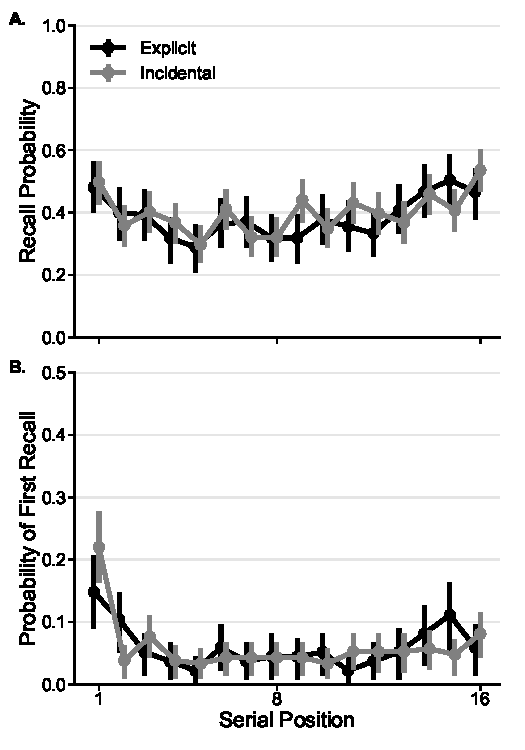
\includegraphics{figures/E2_spc_list2.pdf}
\caption{(A) Serial Position Curves and (B) Probability of First Recall curves on the second list under explicit versus incidental encoding using the Front Door task (Experiment 2). \spcpaneltext}
\label{e2_l2_spc}
\end{figure}


%#####################
%####### E2l1 crp ####
%#####################
\begin{figure}%[hp]
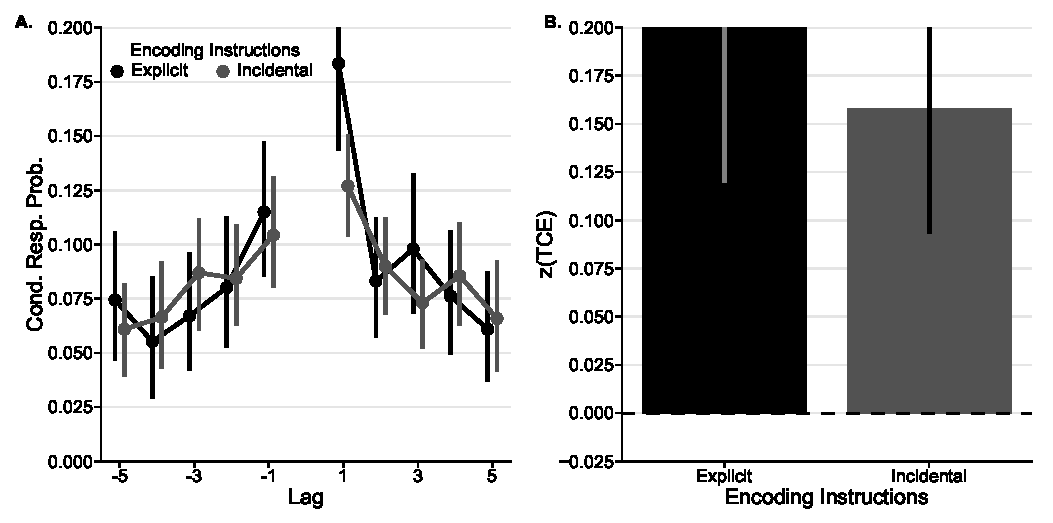
\includegraphics{figures/E2_crp_list2.pdf}
\caption{The temporal contiguity effect (TCE) on the second list under explicit versus incidental encoding using the Front Door task (Experiment 2). \paneltext}
\label{e2_l2_crp}
\end{figure}



%#####################
%####### 3l1 spc ####
%#####################
\begin{figure}
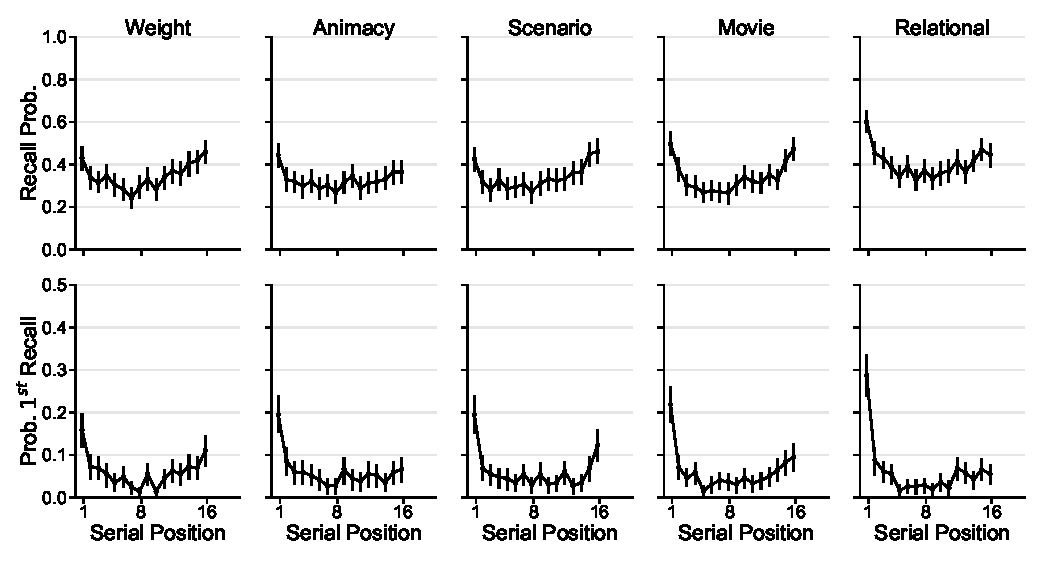
\includegraphics{figures/E3_spc_list2.pdf}
\caption{(Top row) Serial Position Curves and (Bottom row) Probability of First Recall curves on the second list under incidental encoding with different judgment tasks (Experiment 3). \spcpaneltext}~NOTE: There was no second list in the Varying Size condition.
\label{e3_l2_spc}
\end{figure}



%#####################
%####### 3l1 crp ####
%#####################
\begin{figure}%[hp]
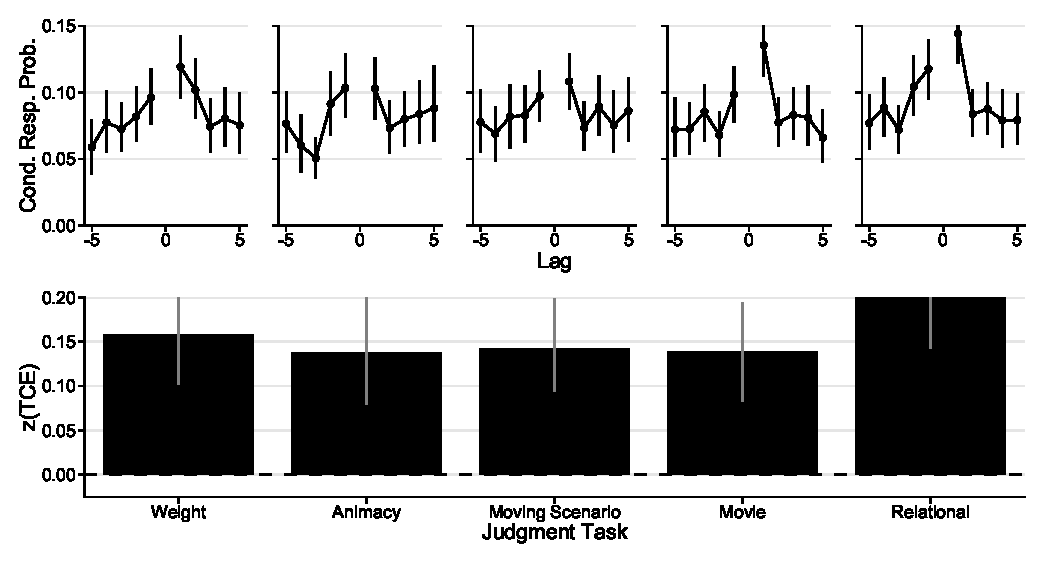
\includegraphics{figures/E3_crp_list2.pdf}
\caption{The temporal contiguity effect (TCE) on the second list under incidental encoding with different judgment tasks (Experiment 3). (Top) Lag-conditional response probability functions. Error bars are bootstrapped within-subject 95\% confidence intervals. (Bottom) The average z(TCE).  Error bars are bootstrapped between-subject 95\% confidence intervals. z(TCE) for a given subject is computed as follows: An observed temporal factor score was computed as the average percentile ranking the temporal lag of each actual transition in the recall sequence with respect to the lags of all transitions that were possible at that time. To determine the temporal factor score expected by chance, a permutation distribution was created by randomly shuffling the order of recalls within the sequence 10,000 times and computing a temporal factor score for each shuffling. The reported value, z(TCE), is z-score of the observed temporal factor score within the permutation distribution.~NOTE: There was no second list in the Varying Size condition.}
\label{e3_l2_crp}
\end{figure}

\bibliography{healey_lab}
\end{document}